\chapterimage{chapter-bg.png} % Chapter heading image

\chapter{Plugins}\label{plugins}

Since version 0.10.3, Stellarium's packages include a number of
plug-ins: Angle Measure, Compass Marks, Oculars, Telescope Control, Text
User Interface, Satellites, Solar System Editor, Time Zone, Historical
Supernovae, Quasars, Pulsars, Exoplanets and Observability analysis. All
these plug-ins are ``built-in'' in the standard Stellarium distribution
and DON'T need to be downloaded separately.

\section{Enabling plugins}\label{enabling-plugins}

%\begin{figure}[h]
%\centering\includegraphics{sat_howto_01.jpg}
%\end{figure}

To enable a plugin:

\begin{enumerate}
\item
  Open the \textbf{Configuration dialog} (press F2 or use the left tool
  bar button)
\item
  Select the \textbf{Plugins} tab
\item
  Select the plugin you want to enable from the list
\item
  Check the \textbf{Load at startup} option
\item
  Restart Stellarium
\end{enumerate}

If the plugin has configuration options, the \textbf{configuration}
button will be enabled when the plugin is loaded and clicking it will
open the plugin's configuration window.

\section{Data for plugins}\label{data-for-plugins}

Some plugins contain files with different data, e.g. catalogs. JSON is a
typical format for those files and you can edit it's manually. Of
course, each plugin has specific format of data for the own catalogs and
you should read documentation for plugin before editing of it catalog.

You can read some common instructions for editing catalogs of plugins
below. In this example we use \texttt{catalog.json} file for
identification of catalog for typical plugin.

You can modify the \texttt{catalog.json} files manually using a text
editor. \textbf{If you are using Windows, it is strongly recommended to
use an advanced text editor such as
\href{http://notepad-plus-plus.org/}{Notepad++}} to avoid problems with
end-of-line characters. (It will also color the JSON code and make it
easier to read.)

\textbf{Warning}: Before editing your \texttt{catalog.json} file, make a
backup copy. Leaving out the smallest detail (such as a comma or
forgetting to close a curly bracket) will prevent Stellarium from
starting.

The path to the directory which contains \texttt{catalog.json} file is
something like:

\section{How you can help}\label{how-you-can-help}

We are welcome bug reports, feature requests and feedback through the
usual channels (trackers, forums and so on).

\chapterimage{chapter-bg.png} % Chapter heading image

\chapter{Built-in plugins}\label{built-in-plugins}

\section{Angle Measure Plugin}\label{angle-measure-plugin}

%\url{http://porpoisehead.net/images/plugin-angle-measure.jpg}

The Angle Measure plugin is a small tool which is used to measure the
angular distance between two points on the sky. *goes misty eyed* I
recall measuring the size of the Cassini Division when I was a student.
It was not the high academic glamor one might expect... It was cloudy...
It was rainy... The observatory lab had some old scopes set up at one
end, pointing at a \emph{photograph} of Saturn at the other end of the
lab. We measured. We calculated. We wished we were in Hawaii. A picture
is worth a thousand words.

\subsection{Using plugin}\label{using-plugin}

\begin{enumerate}
\item
  Enable the tool by clicking the tool-bar button, or by pressing
  \textbf{control-A}. A message will appear at the bottom of the screen
  to tell you that the tool is active.
\item
  Drag a line from the first point to the second point using the left
  mouse button
\item
  To clear the measurement, click the right mouse button
\item
  To deactivate the angle measure tool, press the tool-bar button again,
  or press \textbf{control-A} on the keyboard.
\end{enumerate}

\subsection{Plugin's home page}\label{plugins-home-page}

\url{http://www.stellarium.org/wiki/index.php/AngleMeasure_plugin}

\section{Bright Novae Plugin}\label{bright-novae-plugin}

The Bright Novae plugin provides visualization of some bright novae in
the Milky Way galaxy.

Example (\href{http://en.wikipedia.org/wiki/V1500_Cygni}{\textbf{Nova
Cygni 1975}}, also known as \textbf{V1500 Cyg}):

\begin{figure}[h]
\centering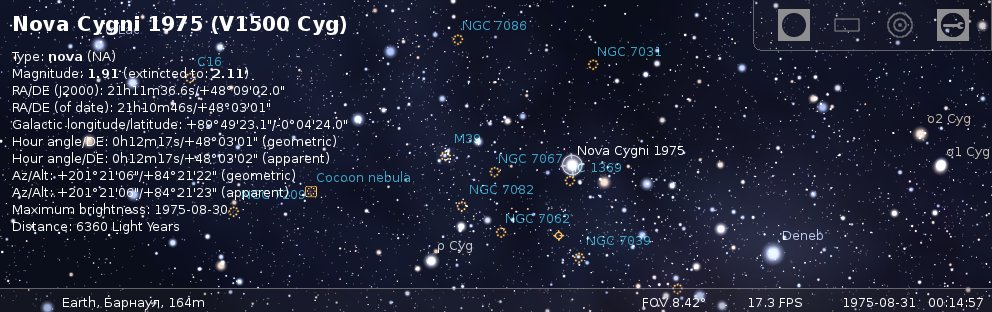
\includegraphics[scale=0.6]{NovaCygni1975wiki.jpg}
\end{figure}

\subsection{Using the Bright Novae plugin}\label{Using-bright-novae-plugin}

\begin{enumerate}
\item
  Enable the tool by clicking the tool-bar button ``Load at startup''
\item
  Set date and time (30 August 1975 year for \emph{Nova Cygni 1975} as
  example)
\end{enumerate}

\subsection{Section \big[Novae\big] in config.ini
file}\label{section-novae-in-config.ini-file}

You can edit \texttt{config.ini} file by yourself for changes of the
settings for the Bright Novae plugin - just make it carefully!

\begin{longtabu} to \textwidth {l|l|X}
\toprule
\emph{ID} & \emph{Type} & \emph{Description}\tabularnewline
\midrule
last\_update & string & Date and time of last update\tabularnewline
\midrule
update\_frequency\_days & int & Frequency of updates, in days\tabularnewline
\midrule
updates\_enable & bool & Enable updates of bright novae catalog from Internet \tabularnewline
\midrule
url & string & URL of bright novae catalog \tabularnewline
\bottomrule
\end{longtabu}

\subsection{Format of catalog of bright novae}\label{format-of-catalog-of-bright-novae}

To add a new nova, open a new line after line 5 and paste the following,
note commas and brackets, they are important:

\begin{config}
\begin{verbatim}
"Nova designation":
{
    "name": "name of nova",
    "type": "type of nova",
    "maxMagnitude": value of maximal visual magnitude,
    "minMagnitude": value of minimal visual magnitude,
    "peakJD": JD for maximal visual magnitude,
    "m2": Time to decline by 2mag from maximum (in days),
    "m3": Time to decline by 3mag from maximum (in days),
    "m6": Time to decline by 6mag from maximum (in days),
    "m9": Time to decline by 9mag from maximum (in days),
    "distance": value of distance between nova and 
                Earth (in thousand of Light Years),
    "RA": "Right ascension (J2000)",
    "Dec": "Declination (J2000)"
},
\end{verbatim}
\end{config}

\newpage
For example, record for \textbf{Nova Cygni 1975} (\textbf{V1500 Cyg}):

\begin{config}
\begin{verbatim}
"V1500 Cyg":
{
    "name": "Nova Cygni 1975",
    "type": "NA",
    "maxMagnitude": 1.69,
    "minMagnitude": 21,
    "peakJD": 2442655,
    "m2": 2,
    "m3": 4,
    "m6": 32,
    "m9": 263
    "distance": 6.36,
    "RA": "21h11m36.6s",
    "Dec": "48d09m02s"
},
\end{verbatim}
\end{config}

\subsection{Light curves}\label{light-curves}

This plugin uses a very simple model for calculation of light curves for
novae stars. This model is based on time for decay by \emph{N}
magnitudes from the maximum value, where \emph{N} is 2, 3, 6 and 9. If a
nova has no values for decay of magnitude then this plugin will use
generalized values for it.

\subsection{Plugin's home page}\label{plugins-home-page-1}

\url{http://www.stellarium.org/wiki/index.php/Bright_Novae_plugin}

\section{Compass Marks Plugin}\label{compass-marks-plugin}

%\url{http://porpoisehead.net/images/plugin-compass-marks.jpg}

Stellarium helps the user get their bearings using the cardinal point
feature - the North, South, East and West markers on the horizon.
Compass Marks takes this idea and extends it to add markings every few
degrees along the horizon, and includes compass bearing values in
degrees.

\subsection{Using plugin}\label{using-plugin-2}

There is a tool bar button for toggling the compass markings, or you can
press \textbf{control-C}.

Note that when you first enable compass marks, the cardinal points will
be turned off. You can have both active at once, but there is a small
bug which means you have to press \textbf{Q} \emph{two times} to
re-enable cardinal points after enabling the compass markings.

\subsection{Plugin's home page}\label{plugins-home-page-2}

\url{http://www.stellarium.org/wiki/index.php/CompassMarks_plugin}

\section{Text User Interface Plugin}\label{text-user-interface-plugin}

%\url{http://porpoisehead.net/images/plugin-tui.jpg}

Older versions of Stellarium used to have a little menu system which was
controlled by the cursor keys. This was used primarily by planetarium
system operators to change settings, run scripts and so on. In the
0.10.x series, this function vanished as we totally re-designed the user
interface. This plugin re-implements the ``TUI'', as it was known. Full
list of the commands for the TUI plugin you can read in the section
\href{TUI_Commands}{TUI Commands}.

\subsection{Using plugin}\label{using-plugin-3}

\begin{enumerate}
\item
  Activate the text menu using the \textbf{m} key
\item
  Navigate the menu using the cursors keys.
\item
  To edit a value, press the right cursor until the value you wish to
  change it highlighted with \textgreater{} and \textless{} marks, e.g.
  \textgreater{}3.142\textless{}. Then press the up and down cursors to
  change the value. You may also type in a new value with the other keys
  on the keyboard.
\end{enumerate}

\subsection{Plugin's home page}\label{plugins-home-page-3}

\url{http://www.stellarium.org/wiki/index.php/TextUserInterface_plugin}

